%==============================================================================
% @author Clinton Freeman <freeman@cs.unc.edu>
% @date 2014-05-23
%==============================================================================

\FloatBarrier
\section{Case Study: Melkman's Algorithm}

This section examines using our workbench to animate Melkman's convex hull
algorithm~\cite{melkman1987line}. 

% By providing a concrete example we hope to illuminate the major steps
% required to animate algorithms in general. Before we get started, let us briefly
% examine the algorithm in question.

\subsection{Algorithm Overview}

A \emph{polyline} $P$ is a polygonal chain of vertices $p_1, p_2, \ldots, p_n$
connected by line segments $p_ip_{i+1}$ for $1 \leq i < n$. $P$ is \emph{simple}
if the only intersection between segments is at their shared endpoints.
Melkman's algorithm incrementally computes the convex hull of a simple polyline
in $O(n)$ time. 

The algorithm stores the hull's vertices in a doubly-ended queue (deque) and
maintains the invariant that they are stored in ccw order from head to tail,
starting and ending with the most recent vertex added to the hull. The algorithm
establishes the invariant initially by forming the deque with $p_2, p_1, p_2$ to
represent the convex hull of the first two points. 

% Figure 1.16 shows the first
% three deques for the convex hulls $CH(P_2), CH(P_3)$, and $CH(P_4)$.

Now, suppose we wish to add $p_i$ to the hull. Let $v, w$ be the vertices at the
tail of the deque and $u, v$ be the vertices at the head. Thus, $v$ is the most
recent vertex added to the hull, and we can speak of edges $uv$ and $vw$ as
being at the head and tail of the deque, respectively. 

%See Figure 1.17.

If $p_i$ is not left of $uv$ or inside $uv$, then remove edge $uv$ from the
convex hull by popping the head of the deque; continue until $p_i$ is left of
the edge at the head. Similarly, if $p_i$ is not left of $vw$ or inside $vw$,
then remove edge $vw$ from the convex hull by popping the tail of the deque;
continue until $p_i$ is left of the edge at the tail. Finally, push $p_i$ onto
both the head and tail of the deque to restore the invariant.

%Two vertices will be popped in Figure 1.17.

On the other hand, if $p_i$ is left or inside both $uv$ and $vw$, then we can 
observe that $p_i$ is not on the convex hull: because the polyline from $v$ to
$p_i$ does not cross the polyline from $u$ to $v$ or from $v$ to $w$, $p_i$ can
leave the hull $CH(P_{i-1})$ only by crossing $uv$ or $vw$. Hull $CH(P_{i-1})$
is identical with $CH(P_i)$, and the invariant already holds.

%As in Figure 1.18,

% Figure 1.19 continues the execution begun in Figure 1.16. It shows all of the
% deques and some of the hulls for $CH(P_5)$ through $CH(P_{14})$. Code is listed
% in Figure 1.20.

% It can also be used to compute the convex
% hull of arbitrary point sets if we first sort by $x$ coordinate, breaking ties
% by $y$ coordinate.

% Melkman's algorithm stores the convex hull vertices in a deque, or doubly-ended
% queue - a simple data structure that stores a list of elements and allows you to
% add and remove (by push() and pop()) elements from the front and back of the
% list. Melkman's algorithm maintains the invariant that the vertices of the
% convex hull CH(P\_i) are stored in a deque in ccw order from head to tail,
% starting and endign with the most recent vertex added to the hull.
% 
% Given an oriented line $pq$ and a point $r$, the 2D orientation predicate
% $\textsc{Orient2D}(p, q, r)$ answers the question, ``is $r$ to the left, right,
% or on $pq$?'' It is often written as the sign of the 2-by-2 determinant, $$
% \textsc{Orient2D}(p, q, r) = \textsc{Sign}\left( \begin{vmatrix} p_x-r_x &
% p_y-r_y \\ q_x-r_x & q_y-r_y \end{vmatrix} \right).$$

% Incremental convex hull algorithms construct the hull by examining each input
% point in turn, exploiting structure in the partial hull to help reduce
% computation. 
% Graham and Yao observed that if we know the points in advance, we
% may make our task easier by considering them in sorted order by $x$ coordinate,
% breaking ties by $y$ coordinate. Then point $p_i$ will always be a vertex of the
% convex hull $\text{CH}(P_i)$, and it will either be adjacent to $p_{i-1}$ or
% will cause $p_{i-1}$ to be removed from $\text{CH}(P_i)$.
 
% \begin{mdframed}[linecolor=white, backgroundcolor=algback, frametitle={Algorithm
% Melkman}] 
% \begin{algorithmic}[1]    
%     \Require Simple polyline $P = \langle v_1, \ldots, v_m \rangle$.
%     \Ensure $\text{CH}(P)$.
%     \vspace{0.75em}
%     \Procedure{Melkman}{$P$}
%     \State $H.push\_back(v_2); H.push\_back(v_1); H.push\_back(v_2);$
%     \Comment{Init hull}
%     \For{$i=3\ldots m$}
%     	\If{\textsc{!LeftOrInside}$(H.back(1), H.back(0), v_i)$ or
%     	\textsc{!LeftOrInside}$(v_i, H.front(1), H.front(0))$} 
%     		\While{\textsc{!LeftOrInside}$(H.back(1), H.back(0), v_i)$}
%     			\State $H.pop\_back();$
%     		\EndWhile
%     		\While{\textsc{!LeftOrInside}$(v_i, H.front(1), H.front(0))$}
%     			\State $H.pop\_front();$
%     		\EndWhile
%     		\State $H.push\_back(v_i);$
%     		\State $H.push\_front(v_i);$
%     	\EndIf
%     \EndFor
%     \State \Return $H$
%     \EndProcedure
% \end{algorithmic}
% \end{mdframed} 

% Animating an algorithm using the workbench is composed of a number of tasks,
% namely 
% \begin{itemize}
%   \item Implement input data structures and instrument them with visualization
%   code.
%   \item Optionally modify the GUI to allow the user to create instances of
%   the input data structure.
%   \item Implement output data structures and instrument them with visualization
%   code.
%   \item Implement predicates.
%   \item Implement the algorithm and instrument it with a small amount of
%   visualization code.
%   \item Optionally modify the GUI to allow the user to run the algorithm on
%   selected input data. 
% \end{itemize}

% \subsection{Data Structures}
% 
% polychain\_2r
% 
% polygon\_2r

\subsection{Algorithm Implementation}

The code listed below shows the \texttt{Melkman} function which is our C++
implementation of Melkman's algorithm. The function takes as input a
\texttt{Polyline\_2r} and an \texttt{IGeometryObserver}, and produces as output
a \texttt{Polygon\_2r} object. All branching tests make use of the
\texttt{RIsLeftOrInsidePQ} predicate, which encapsulates the logic described in
the previous section. We will describe each of these in the paragraphs that
follow.
 
\lstinputlisting{code-samples/melkman.cpp} 

The \texttt{Polyline\_2r} class uses a deque to store its vertices. The
\texttt{push\_back} and \texttt{pop\_back} methods are responsible for
visualizing how those operations affect the visual state of the object.

\lstinputlisting{code-samples/polyline.cpp}

\lstinputlisting{code-samples/polyline-push-back.cpp}

The \texttt{Polygon\_2r} class is composed of a \text{Polyline\_2r} boundary
that is responsible for visualizing vertices and edges. It can optionally
visualize the polygon interior by triangulating it into a fan.  

\lstinputlisting{code-samples/polygon.cpp}  
 
\subsection{Generating Input Data} 

Create button and implement click handler. buttongroup to model mutually
exclusive input states.

define input states. configmanager singleton. 


Handle ortho widget mouse clicks
forward signals from ortho to scene observer

\begin{figure}[h]
	\centering
	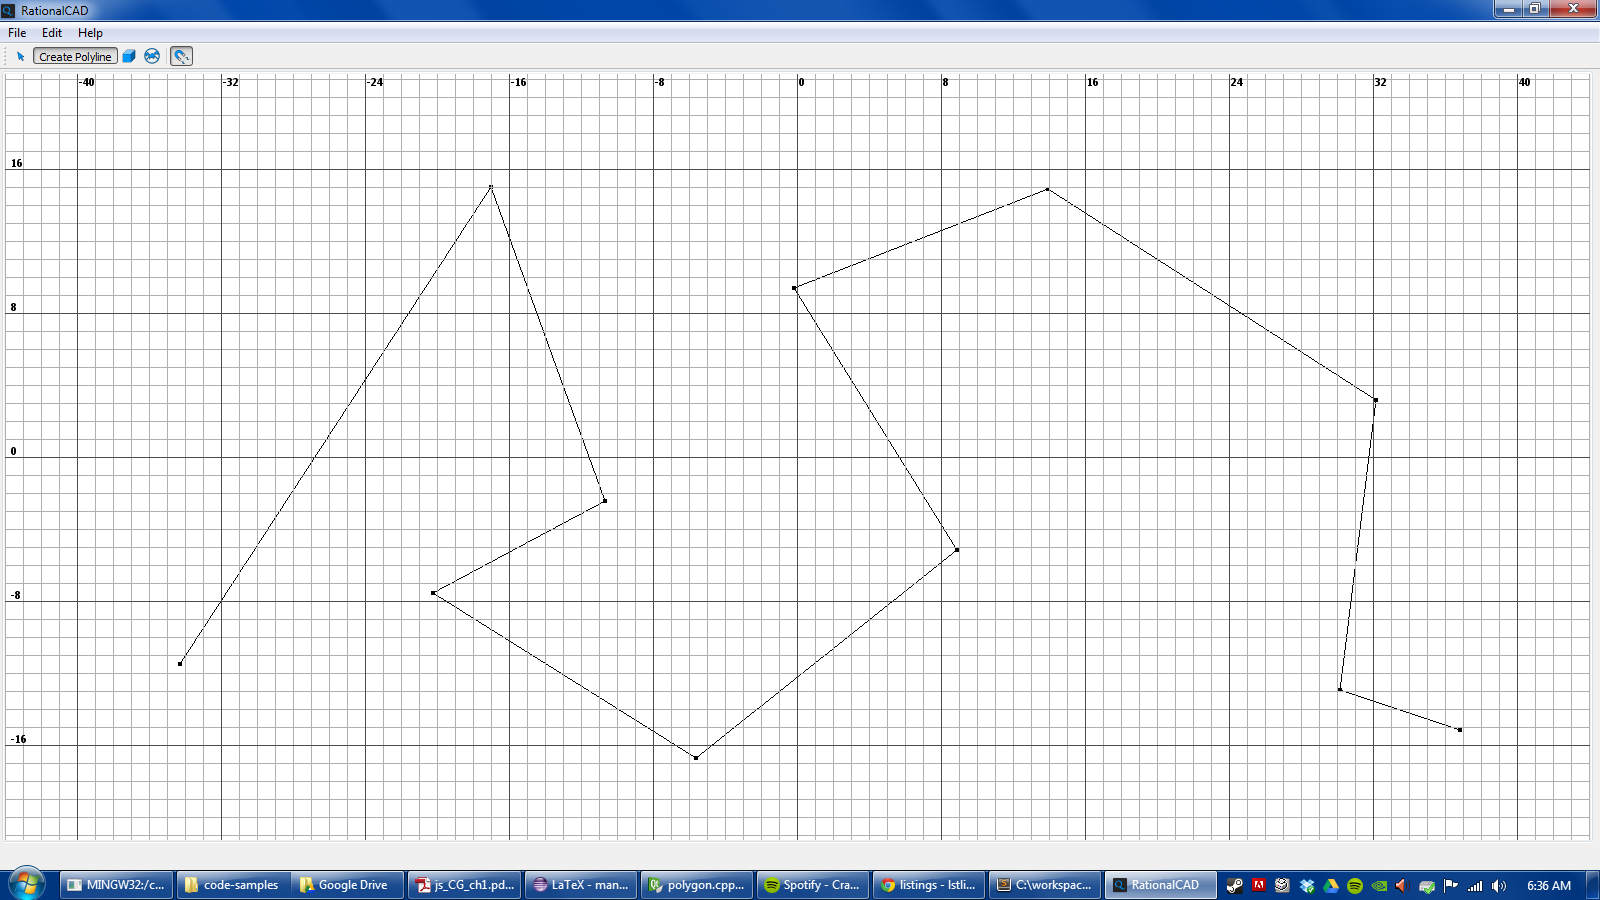
\includegraphics[width=\textwidth]{figures/melkman-input-1}
	\caption{Example polyline input.}
	\label{fig:melkman-input}
\end{figure}




% Animating any algorithm begins with generating the appropriate input. In the
% case of Melkman's algorithm, we begin by creating a simple polyline. This is
% accomplished by the user clicking on points in the 2D top-down orthographic
% view. The user may choose to place integer vertex coordinates or turn off
% snapping so that vertex coords are floating point or rational coords.
% 
% 
% 
% \begin{lstlisting}
% Polygon_2r Melkman(const PolyChain_2r& P, Visual::IGeometryObserver* ge_obs) {
%     Polygon_2r CH_P;
% 
% 
%     return CH_P;
% }
% \end{lstlisting}